\section*{Question 3}
I just wrote a function that create the portfolios and calculate the portfolio return based on "Equal" and "Market" weighting. The function is shown in the code \ref{pcode:3a}. The function takes the following inputs:
\begin{itemize}
    \item \textbf{df}: The dataframe that contains the data
    \item \textbf{sorting\_car}: The variable that will be used to sort the stocks
    \item \textbf{number\_of\_portfolios}: The number of portfolios that will be created
    \item \textbf{weighting}: The type of weighting that will be used to calculate the portfolio return. The default is "Equal" weighting.
\end{itemize}

\begin{lstlisting}[language=Python, caption= Python function to create portfolios, label={pcode:3a}, escapechar=|, frame=single, basicstyle=\small, showstringspaces=false, captionpos=b, breaklines=true, showspaces=false, showtabs=false, keywordstyle=\color{blue}, commentstyle=\color{gray}]
    def get_portfolios(df, sorting_car, number_of_portfolios,weighting = 'Equal'):
    portfoli_df = df.dropna(subset=[sorting_car])[
        ['t', 'permno', sorting_car, 'me', 'ret']
    ].copy()
    portfoli_df['portfolios'] = portfoli_df.groupby('t')[sorting_car].transform(lambda x: pd.qcut(x, number_of_portfolios, labels=False)) 
    portfoli_df['portfolios'] = portfoli_df['portfolios'] + 1   # The highest value is the highest portfolio
    if weighting == 'market':
        portfoli_df['weight'] = portfoli_df.groupby(['t','portfolios'])['me'].transform(lambda x: x/sum(x))
        portfoli_df['ret'] = portfoli_df['ret'] * portfoli_df['weight']
    elif weighting == 'Equal':
        portfoli_df['weight'] = portfoli_df.groupby(['t','portfolios'])['me'].transform(lambda x: 1/len(x))
        portfoli_df['ret'] = portfoli_df['ret'] * portfoli_df['weight']
    return portfoli_df.groupby(['t','portfolios']).ret.sum().unstack().reset_index().rename(columns = {"t":"month"})
\end{lstlisting}

\begin{enumerate}[(a)]
\item Here is the result of the function for the "Equal" weighting. (Figure \ref{fig:3a}) As we can see, at the beginning of the sample, all the portfolios have the same return. However, as time goes by, the return of the portfolios start to diverge. At the end of the sample, the cumulative return of the highest portfolio is much lower than the lowest portfolio. 
\begin{figure}[htbp!]
    \centering
    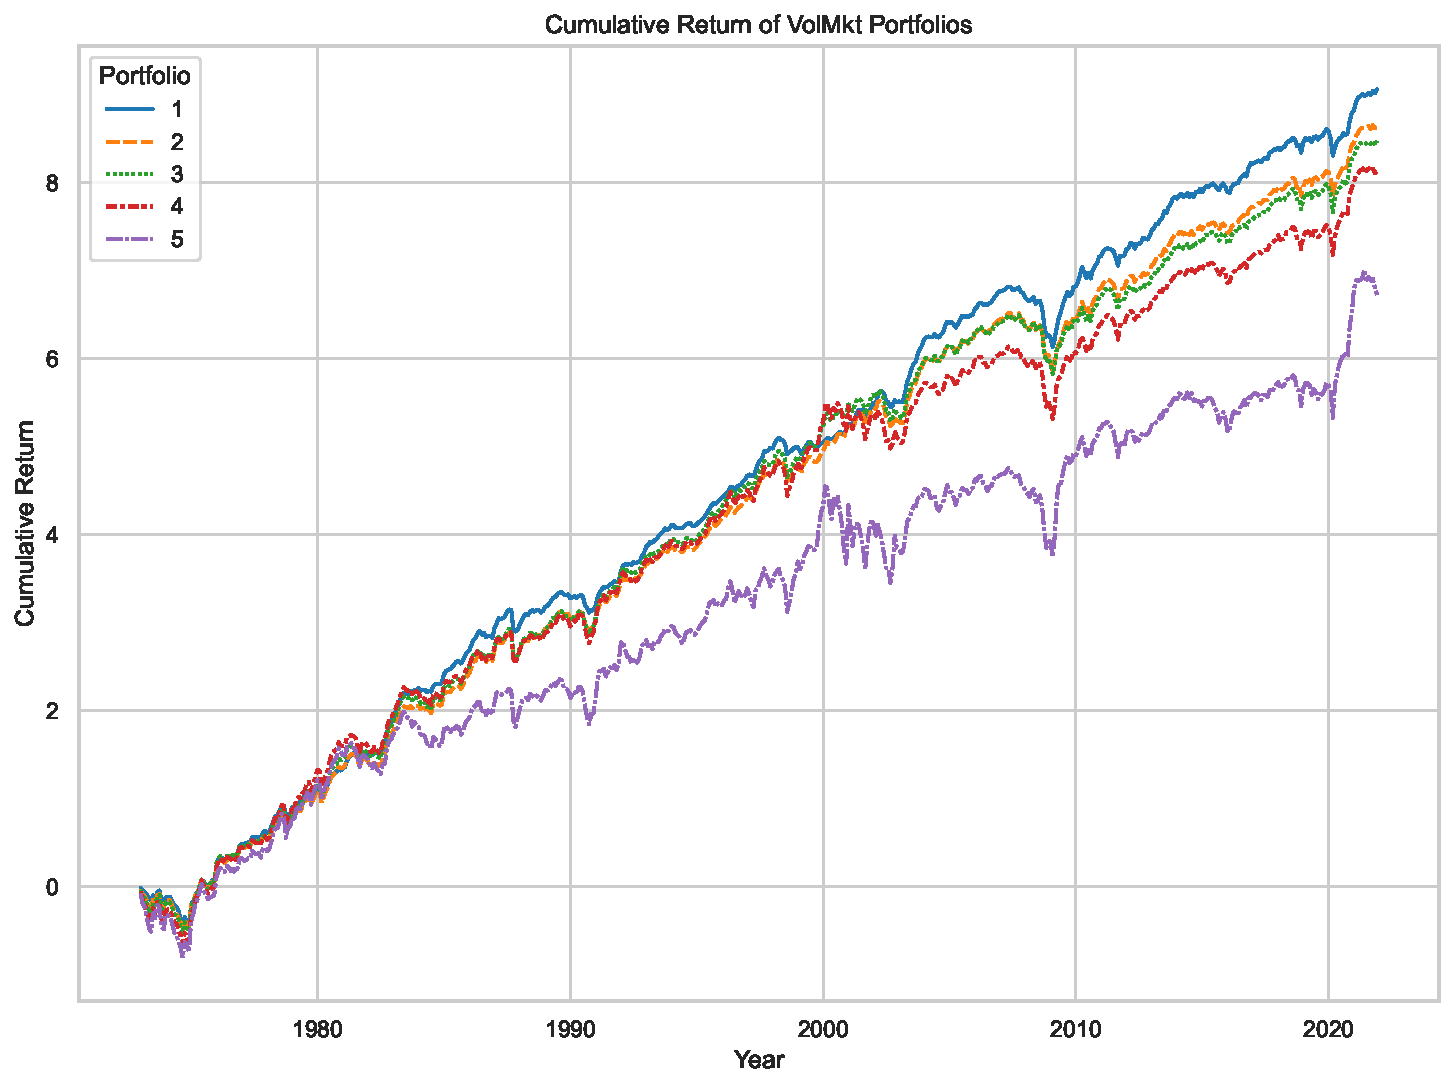
\includegraphics[width=0.6\textwidth]{Out/3_1.pdf}
    \caption{Time series of the average returns of the portfolios based on the "Equal" weighting.}
    \label{fig:3a}
\end{figure}

\item Here is the result of the function for the "Market" weighting. (Figure \ref{fig:3b}) As we can see, the market weighting does not have the same pattern as the "Equal" weighting. The return of the portfolios are stay close to each other and do not diverge as much as the "Equal" weighting. In fact, the cumulative return of the highest portfolio is higher than the lowest portfolio which is the opposite of the "Equal" weighting. I report the average return of the portfolios in the table \ref{tab:3b}.
\begin{figure}
    \centering
    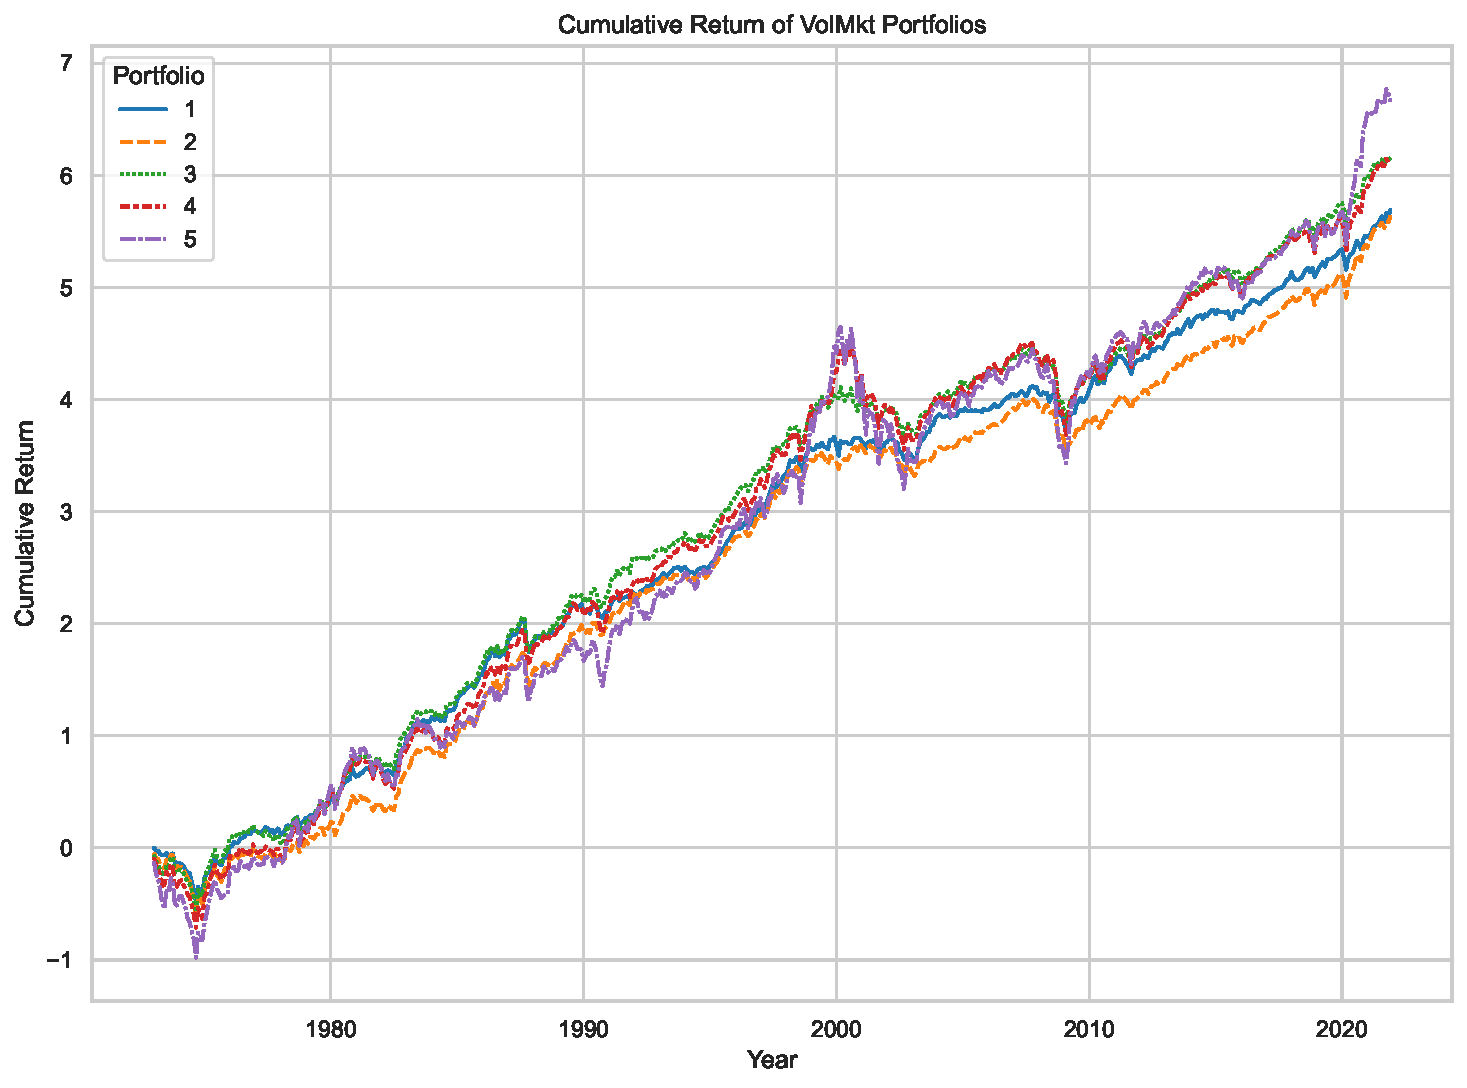
\includegraphics[width=0.6\textwidth]{Out/3_2.pdf}
    \caption{Time series of the average returns of the portfolios based on the "Market" weighting.}
    \label{fig:3b}
\end{figure}

\begin{table}[htbp!]
    \centering
    \caption{Average returns of the portfolios with different weighting}
    \label{tab:3b}
    \begin{tabular}{lrrrrr}
\toprule
portfolios &  Lowest &      2 &      3 &      4 &  Highest \\
\midrule
Equal Weighted  &  0.0154 & 0.0147 & 0.0144 & 0.0138 &   0.0114 \\
Market Weighted &  0.0097 & 0.0096 & 0.0105 & 0.0104 &   0.0113 \\
\bottomrule
\end{tabular}

\end{table}

\item Here we create the long-short portfolio. The long-short portfolio is created by taking the difference between the returns of the highest and the lowest portfolio. The result is shown in the figure \ref{fig:3c}. As we can see, the long-short portfolio has a positive return for the equal weighting and a negative return for the market weighting.

\begin{figure}[htbp!]
    \centering
    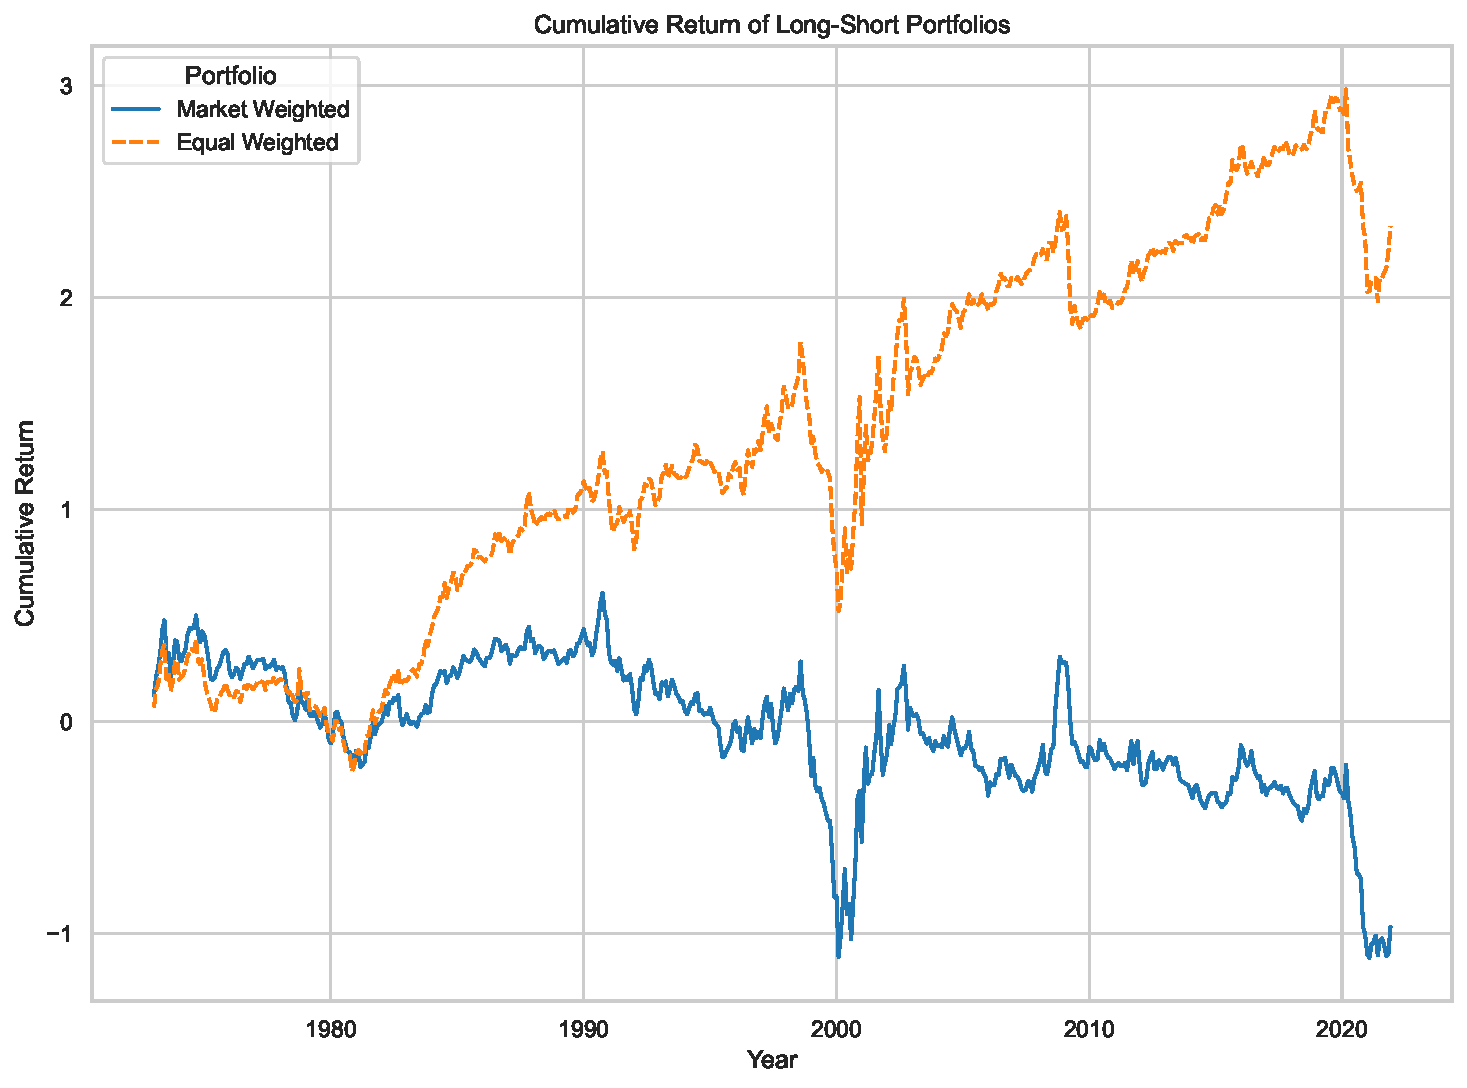
\includegraphics[width=0.6\textwidth]{Out/3_3.pdf}
    \caption{Time series of the average returns of the long-short portfolio.}
    \label{fig:3c}
\end{figure}

Now we can test the CAPM, Fama-French 3 factors and the Fama-French 5 factors, Carhart, and HXZ models. You can find the function that I write to test the null hypothesis that $\alpha_{LS} =0$. I will use the Newey-West standard errors to test the null hypothesis. The result of the test is shown in the table \ref{tab:3c}.


\begin{lstlisting}[language=Python, caption= Python function to run the test, label={pcode:3a}, escapechar=|, frame=single, basicstyle=\small, showstringspaces=false, captionpos=b, breaklines=true, showspaces=false, showtabs=false, keywordstyle=\color{blue}, commentstyle=\color{gray}]
    def time_series_regression(portfolios, factors, FactorModel):
    portfolios = portfolios.merge(factors, on='month', how='left')
    portfolios = portfolios.dropna()
    X = portfolios[FactorModel]
    X = sm.add_constant(X)
    Y = portfolios['long_short']
    model = sm.OLS(Y, X).fit(cov_type='HAC',cov_kwds={'maxlags':int(len(Y)**0.25)}) 
    pvalues = model.pvalues
    betas = model.params
    return [betas.iloc[0],pvalues.iloc[0]]
\end{lstlisting}

You can find the result of the test in the table \ref{tab:3c} for CAPM, Fama-French 3 factors, Fama-French 5 factors, Carhart, and HXZ models. 
\begin{table}[htbp!]
    \caption{$\alpha$ test for long-short portfolio with different models}
    \label{tab:3c}
    \begin{tabularx}{\linewidth}{CC}
        \caption*{Equal Weighted }
        \begin{tabular}{lcc}
\toprule
 & $\alpha$ & $Pvalue$ \\
\midrule
CAPM & 0.010 & 0.000 \\
FF3 & 0.008 & 0.000 \\
CAR & 0.003 & 0.167 \\
FF5 & 0.003 & 0.167 \\
HXZ & 0.000 & 0.944 \\
\bottomrule
\end{tabular}

        &
        \caption*{Market Weighted }
        \begin{tabular}{lcc}
\toprule
 & $\alpha$ & $Pvalue$ \\
\midrule
CAPM & 0.004 & 0.073 \\
FF3 & 0.002 & 0.267 \\
CAR & -0.000 & 0.790 \\
FF5 & -0.003 & 0.061 \\
HXZ & -0.004 & 0.036 \\
\bottomrule
\end{tabular}

    \end{tabularx}
\end{table}
\item 
Now we can test the long-short portfolio for in and out of sample. The result is shown in the table \ref{tab:3d1} for the equal weighting and in the table \ref{tab:3d2} for the market weighting. As we can see, the $\alpha$ is statistically different from zero for the equal weighting for the sample period and the post-publication period except for the HXZ model. For the market weighting, the $\alpha$ is not statistically different from zero for the sample period and the post-publication period as well.
\begin{table}[htbp]
    \caption{$\alpha$ test long-short portfolio for in and out of sample with equal weighting}
    \label{tab:3d1}
    \begin{tabularx}{\linewidth}{CC}
        \caption*{Sample period }
        \begin{tabular}{lcc}
\toprule
 & $\alpha$ & $Pvalue$ \\
\midrule
CAPM & 0.010 & 0.000 \\
FF3 & 0.008 & 0.000 \\
CAR & 0.006 & 0.008 \\
FF5 & 0.005 & 0.016 \\
HXZ & 0.005 & 0.081 \\
\bottomrule
\end{tabular}

        &
        \caption*{Post-publication period}
        \begin{tabular}{lcc}
\toprule
 & $\alpha$ & $Pvalue$ \\
\midrule
CAPM & 0.012 & 0.002 \\
FF3 & 0.011 & 0.000 \\
CAR & 0.007 & 0.027 \\
FF5 & 0.005 & 0.132 \\
HXZ & 0.001 & 0.777 \\
\bottomrule
\end{tabular}

    \end{tabularx}
\end{table}

\begin{table}[htbp]
    \caption{$\alpha$ test long-short portfolio for in and out of sample with market weighting}
    \label{tab:3d2}
    \begin{tabularx}{\linewidth}{CC}
        \caption*{Sample period }
        \begin{tabular}{lcc}
\toprule
 & $\alpha$ & $Pvalue$ \\
\midrule
CAPM & 0.004 & 0.089 \\
FF3 & 0.002 & 0.346 \\
CAR & 0.000 & 0.911 \\
FF5 & -0.000 & 0.896 \\
HXZ & -0.001 & 0.821 \\
\bottomrule
\end{tabular}

        &
        \caption*{Post-publication period}
        \begin{tabular}{lcc}
\toprule
 & $\alpha$ & $Pvalue$ \\
\midrule
CAPM & 0.005 & 0.115 \\
FF3 & 0.004 & 0.056 \\
CAR & 0.002 & 0.286 \\
FF5 & -0.002 & 0.389 \\
HXZ & -0.003 & 0.198 \\
\bottomrule
\end{tabular}

    \end{tabularx}
\end{table}


\end{enumerate}